%!TEX root = ../../../root.tex

\begin{figure}[H]
	\centering
	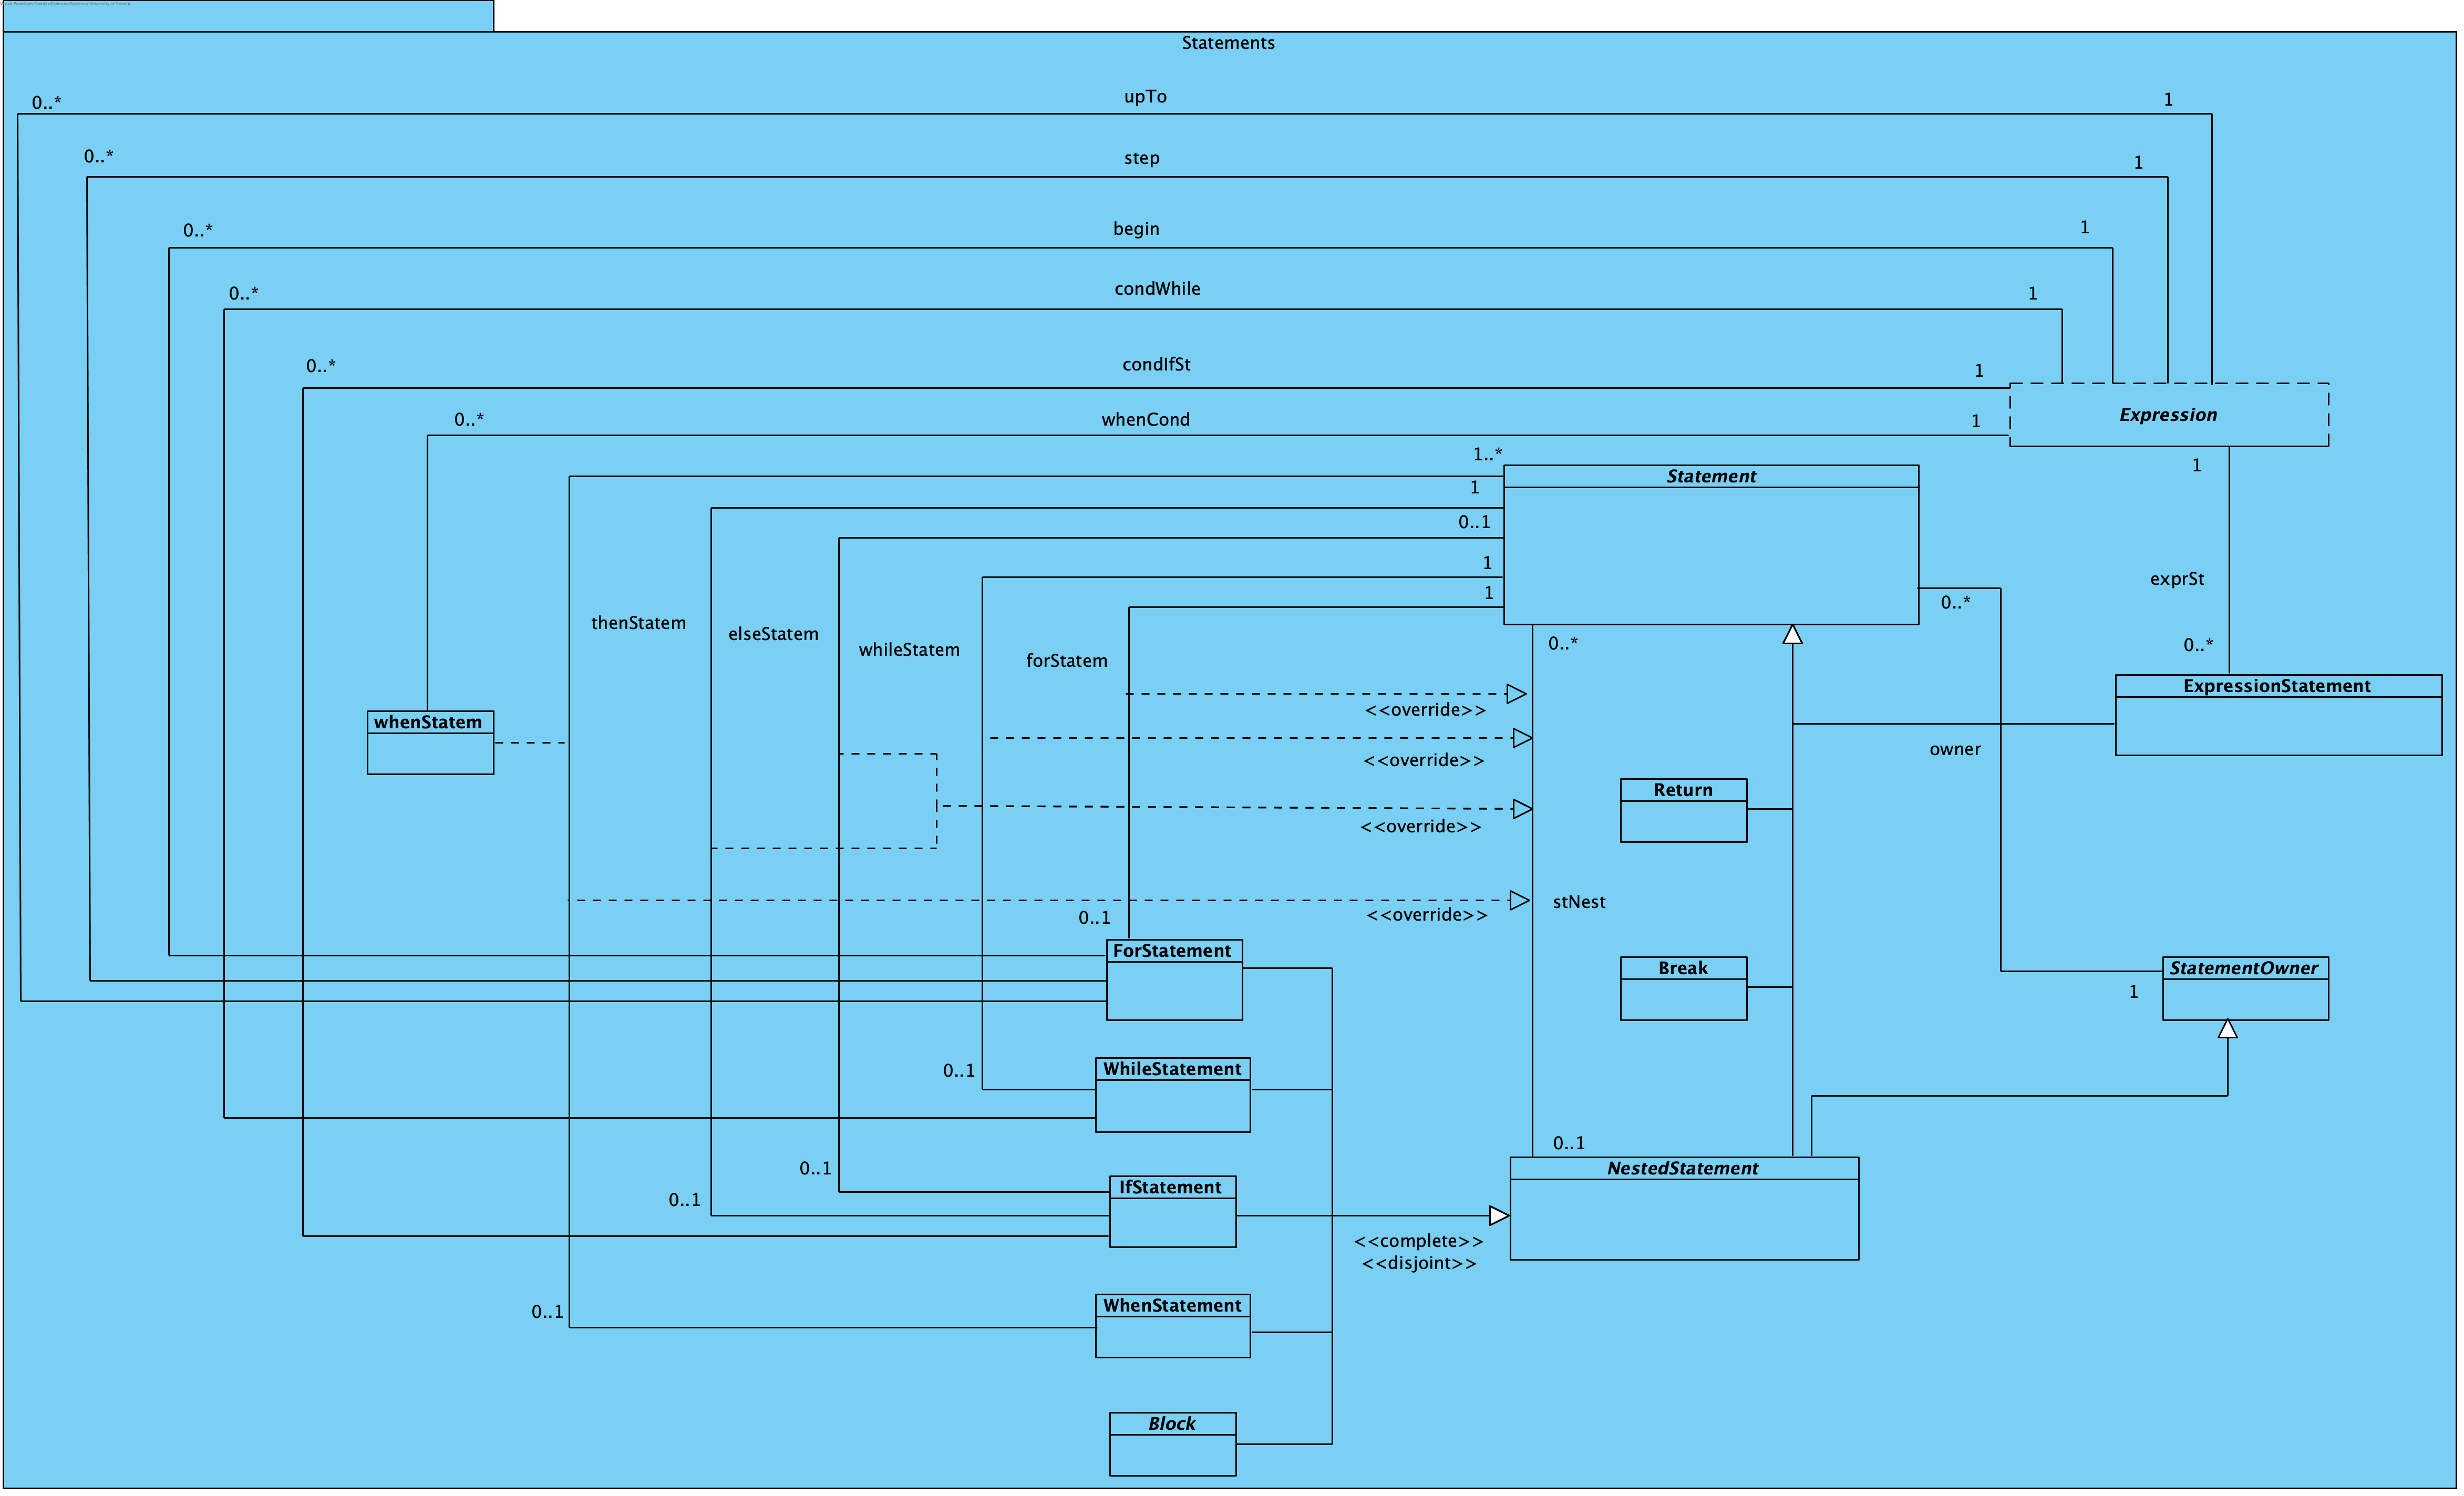
\includegraphics[width=\textwidth]{StatementsAnalysis.png}
	\caption{\small{\textit{Conceptual Analysis: Package Statements.}}}
\end{figure}
\small{\textit{Nota: Le classi con i bordi tratteggiati appartengono ad un package differente dal seguente.}}

\InputSection[sec:modelstranslator:analysis:statements_analysis:stereotypes]{Stereotipi}{Stereotypes/content.tex}
\InputSection[sec:modelstranslator:analysis:statements_analysis:statement]{Classe Statement}{Statement/content.tex}
\InputSection[sec:modelstranslator:analysis:statements_analysis:statementowner]{Classe StatementOwner}{StatementOwner/content.tex}
